%-*-coding: utf-8-*-
\chapter{Теоретическое решение}

\section{Предобработка данных}

Для решения поставленной задачи первым делом необходимо построить
навигационный граф. Подразумевается, что карта содержит множество
контуров, которые можно классифицировать на ограничивающие воду и
ограничивающие сушу. Контура заданы как последовательности точек в
плоской проекции Меркатора~\cite{thomas1952conformal}. Для построения
графа выполняется определённый набор действий.

Первым делом происходит упрощение водных контуров, полученных из карты, и
объединение их в один полигон. Упрощение выполняется по двум причинам:
\begin{itemize}
    \item Хоть такая модификация и может повлиять на корректность
      маршрута, действительно сильно некорректных маршрутов от неё
      появиться не может. Неформальная постановка задачи допускает
      такие модификации. Кроме того, планируется искать маршруты по
      всему земному шару, поэтому мелкомасштабные детали не несут
      никакой информации.
    \item Данные с мелкомасштабной морской карты содержат слишком
      много точек, из-за чего в навигационном графе будет крайне много
      вершин и рёбер, если не упрощать контура. Это приведёт к тому,
      что граф будет занимать слишком много памяти, а поиск путей в
      нём будет занимать слишком много времени.
\end{itemize}
Для упрощения используется алгоритм Дугласа-Пекера~\cite{douglas1973algorithms}.

После построения единого полигона, описывающего контуры воды, для него
строится straight~skeleton~\cite{aichholzer1996straight}, с помощью
которого выполняется смещение полигона внутрь. Это делается по
следующим причинам:
\begin{itemize}
    \item Корабли, как правило, не плавают слишком близко к суше (в
      двенадцатимильной зоне)~\cite{o1984international}. При этом стоит в
      очередной раз отметить, что в данной задаче не требуется искать
      кратчайший маршрут, а требуется получать естественные маршруты,
      которые потенциально могут использоваться для реальных кораблей.
    \item Маршруты, проходящие по границе суши, хуже визуализируются,
      поскольку перемешиваются с сушей. В то же время при визуализации
      маршрутов, проходящих на небольшом расстоянии от суши, таких
      проблем не возникает.
    \item Такая модификация позволяет нейтрализует возможные нарушения
      корректности маршрута, возникающие из-за упрощения контуров.
      Если при упрощении любая точка смещается на расстояние не больше
      $l$, а смещение контура происходит на расстояние $d > l$, то про
      любую точку, принадлежащую итоговому полигону, можно сказать,
      что в исходной карте она точно принадлежит контуру с водой.
\end{itemize}

По смещённому полигону строится навигационный граф. Для этого на
плоскости, на которую спроецирована карта, строится сетка с некоторым
постоянным шагом. Для каждого ребра сетки проверяется принадлежность
полигону, ограничивающему воду. Если ребро полностью принадлежит
полигону, то оно добавляется в граф (вместе с инцидентным вершинами).
Помимо этого в граф добавляются все вершины полигона и рёбра до
видимых вершин (то есть рёбра, полностью принадлежащие полигону) в
некотором радиусе. При этом важно ограничить максимальную длину ребра.
Это связано с тем, что граф строится по полигону в плоской проекции,
проверка принадлежности отрезка полигону также выполняется в плоской
проекции. В то же время кратчайшее расстояние между двумя точками на
Земле достигается не для отрезка, а для дуги (приближённо). Поэтому
такая проверка, вообще говоря, некорректна. Однако, если ограничить
длину ребра, то отклонение дуги от отрезка будет невелико. Учитывая
то, что полигон смещён внутрь, можно утверждать, что любое ребро
действительно будет проходить по воде, не пересекая препятствия.

Также в полученный граф добавляются дополнительные рёбра. Во-первых,
добавляются рёбра, получившиеся в результате «схлопывания» контуров
полигона при построении straight skeleton'а. При этом они также
упрощаются. Это необходимо сделать, потому что при смещении полигона
некоторые контура «схлопываются», объединяясь в один. Если между ними
был, скажем, какой-нибудь канал, то по нему нельзя будет пройти в
итоговом графе. Именно поэтому такие рёбра из straight skeleton'а
добавляются в граф. Во-вторых, поскольку граф строится по контурам в
проекции Меркатора, то в нём отсутствуют рёбра через 180-ый меридиан.
Такие рёбра также добавляются в граф.

\FloatBarrier

\section{Поиск одного маршрута}

Прежде чем перейти к описанию алгоритма поиска семейств маршрутов,
необходимо детально описать процесс поиска одного маршрута в
построенном навигационном графе. Первым делом для двух заданных точек
проверяется принадлежность полигону, ограничивающему воду. Если точки
действительно находятся на воде, то по имеющейся сетке для них
находятся ближайшие вершины графа, и все корректные рёбра до ближайших
вершин добавляются в граф. После этого используется алгоритм
Дейкстры~{dijkstra1959note} для поиска кратчайшего пути в графе между
этими двумя вершинами. Поиск останавливается, когда кратчайший путь до
нужной вершины найден.

Поскольку найденный путь не является действительно кратчайшим
маршрутом между двумя точками, производится попытка его сократить. Для
каждой вершины пути проверяется, можно ли её убрать из маршрута, не
нарушив его корректность и не увеличив длину пути. Если можно, то
такая вершина убирается из маршрута. Этот процесс может повторяться
несколько раз, для чего каждый отрезок пути разбивается на подотрезки
меньшей длины. После этого опять производится попытка выкинуть точки.
И так далее. Ещё одна модификация маршрута вызвана тем, что в связи со
структурой графа в маршруте могут появляться слишком острые углы (если
в каком-нибудь контуре, образованном при смещении полигона, есть
острый угол). В реальных маршрутах не бывает острых углов, поэтому
выполняется сглаживание маршрута, то есть замена острого угла ломаной,
аппроксимирующей дугу эллипса. При этом корректность такой замены
проверяется по исходному полигону, не смещённому внутрь.

\begin{figure}
    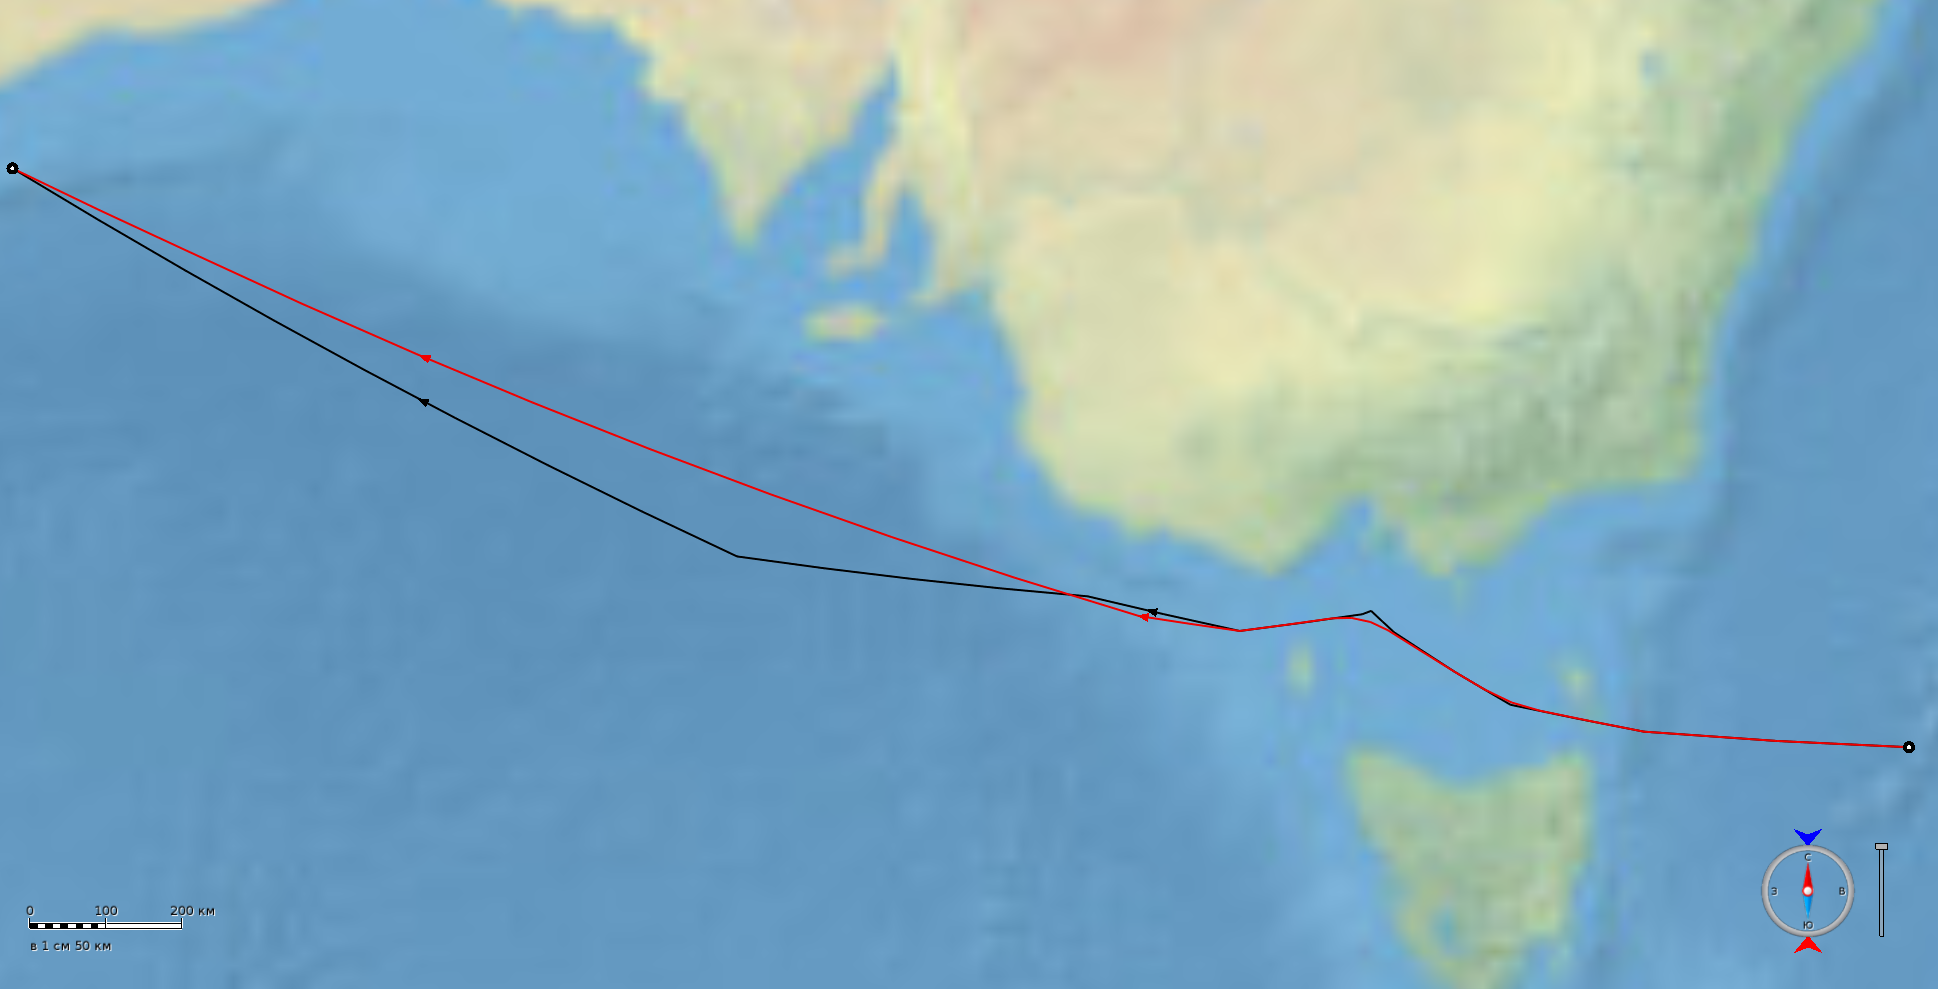
\includegraphics[width=\textwidth]{Solution/shortcut-and-smoothing}
    \caption{Сокращение и сглаживание маршрута}
    \label{fig:path-improvements}
\end{figure}

На рисунке \ref{fig:path-improvements} продемонстрирован эффект от
сокращения и сглаживания маршрута. Чёрной линией изображён кратчайший
путь в графе, а красной --- итоговый маршрут. Нетрудно видеть, что
левая часть маршрута сократилась, а в правой части произошло
сглаживание, что сделало маршрут более естественным.

\FloatBarrier

\section{Поиск нескольких маршрутов}

Для поиска нескольких маршрутов используется итеративный алгоритм. На
рисунке \ref{alg:multipath} представлен псевдокод алгоритма. Первым
делом выполняется поиск первого маршрута описанным выше способом,
найденный маршрут добавляется в результирующее множество, запоминается
его длина. Затем, пока количество найденных маршрутов не достигнет
максимально возможного, выполняются следующие действия: обновление
весов рёбер в графе, поиск очередного маршрута, проверка критерия
остановки. Критерий остановки был сформулирован в формальной
постановке задачи и состоит в том, что длина найденного маршрута
должна быть не более чем в $C_0$ раз больше длины кратчайшего
маршрута, и не один из имеющихся маршрутов не должен быть похожий на
последний найденный. Функция $similar(p, q)$ проверяет, похожи ли
маршруты в соответствии с формализацией, приведённой в постановке
задачи. Практическая реализация этой функции описана в следующей
главе.

Остановимся поподробней на процессе обновления весов. Обновление весов
основано на введении для каждой вершины графа некоторого потенциала.
Чем больше потенциал вершины, тем сильнее увеличиваются веса
инцидентных ей рёбер. Чем ближе вершина к найденному маршруту, тем
сильнее должен увеличиваться вес инцидентных ей рёбер, чтобы
находились непохожие маршруты. Для поиска потенциалов первым делом
строится граф с фиктивной вершиной, из которой проводятся рёбра
нулевого веса во все вершины очередного пути (функция
$graph\_with\_fake$ в псевдокоде). Вводится максимальное расстояние,
равное $\frac{len}{C_1}$, где константа $C_1$ является параметром
алгоритма. Для всех вершин, до которых длина кратчайшего пути в графе
меньше этого расстояния, могут быть увеличины потенциалы. После этого
используется алгоритм Дейкстры для поиска кратчайших расстояний из
фиктивной вершины, при этом поиск заканчивается, когда достигнуто
максимальное расстояние. Кратчайшее расстояние до непосещённых вершин
принимается равным максимальному. Следующий вопрос состоит в
вычислении потенциалов вершин по найденным расстояниям и обновлении
весов рёбер по введённым потенциалам. Наиболее очевидным и простым
решением является вычислять значение потенциала, используя убывающую
линейную функцию от кратчайшего расстояния (например, $\frac{limit -
  dist}{A}$, где $limit$ --- введённое выше максимальное расстояние,
$dist$ --- найденное кратчайшее расстояние от фиктивной вершины,
$A > 0$ --- некоторая константа), и прибавлять к весу ребра среднее
арифметическое потенциалов инцидентных ему вершин. Однако такой подход
обладает определённым недостатком.

\begin{figure}
    \begin{algorithmic}
        \Function{find\_paths}{}
            \State p, len $\gets$ find\_path()
            \State paths $\gets$ {p}
            \State min\_len $\gets$ len
            \While{paths.size() < max\_paths\_count}
                \State update\_weigths(p, len)
                \State p, len $\gets$ find\_path()
                \If{$len > C_0 \cdot min\_len$}
                    \State \Return paths
                \EndIf
                \For{q in paths}:
                    \If{similar(p, q)}
                        \State \Return paths
                    \EndIf
                \EndFor

                \State paths.insert(p)
           \EndWhile
        \EndFunction

        \Function{update\_weights}{p, len}
            \State g' $\gets$ graph\_with\_fake(p)
            \State limit $\gets \frac{len}{C_1}$
            \State d $\gets$ shortest\_in\_radius(g', fake, limit)
            \ForAll{v in p}
                \State d[v] = $\frac{limit}{M}$
            \EndFor
            \ForAll{v in vertices}
                \State potential = $1 + (max\_potential - 1) \cdot \frac{limit - d[v]}{limit}$
                \State potentials[v] = max(potentials[v], potential)
            \EndFor
            \ForAll{e in edges}
                \State e.weight = $e.initial\_weight \cdot
                sqrt(potentials[e.from] \cdot potentials[e.to])$
            \EndFor
        \EndFunction
    \end{algorithmic}
    \caption{Псевдокод поиска нескольких маршрутов}
    \label{alg:multipath}
\end{figure}

\begin{figure}
    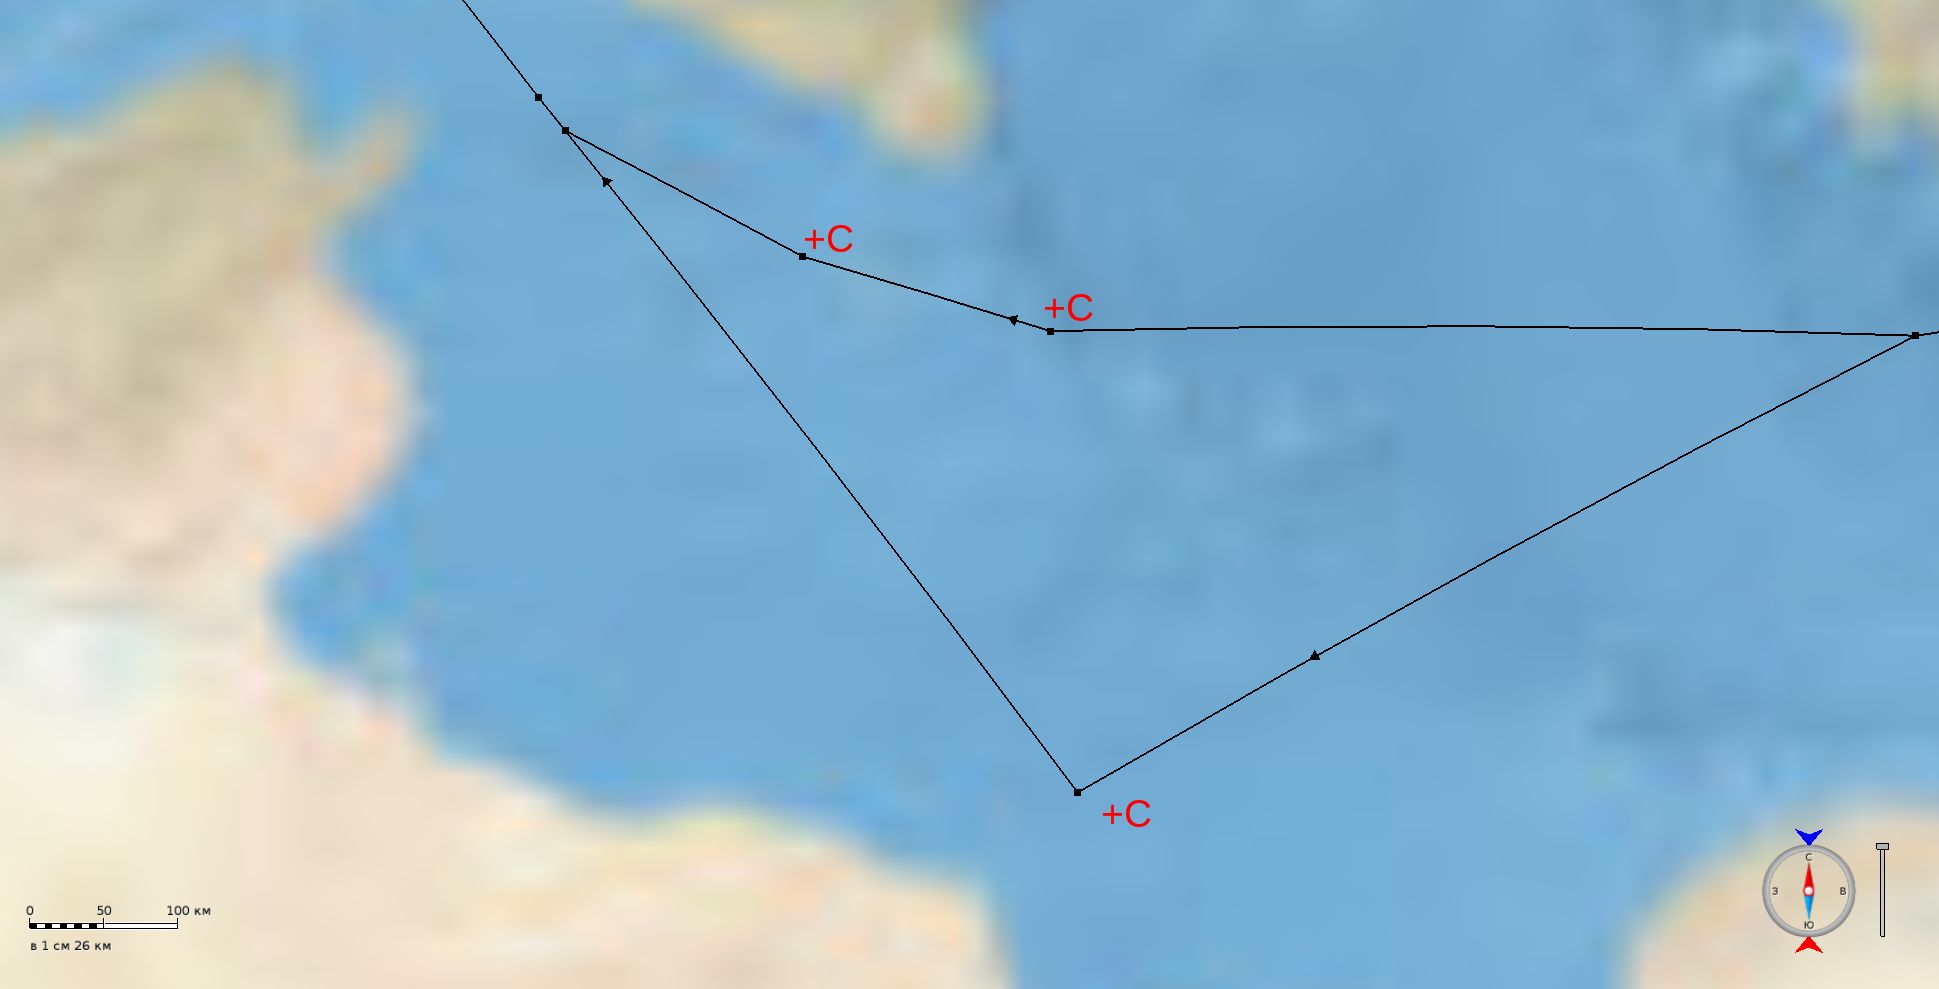
\includegraphics[width=\textwidth, clip=true, trim = 400 0 0
    0]{Solution/potentials-multipliers}
    \caption{Потенциалы должны быть множителями}
    \label{fig:potentials-multipliers}
\end{figure}

Рассмотрим рисунок~\ref{fig:potentials-multipliers}. На данном рисунке
между крайней правой и крайней левой точкой есть два альтернативных
пути. Предположим, что до этого был найдены длинные маршруты (хотя бы
один). В этом случае, поскольку изображённые вершины находятся близко
друг к другу, их потенциалы будут примерно равны некоторому $C$.
Тогда, если использовать предложенный выше подход, то увеличение веса
верхнего пути за счёт потенциалов будет на $C$ больше, чем увеличение
веса нижнего пути. Из-за этого будет выбран более длинный нижний путь.
Таким образом, возникает проблема в том, что вес пути начинает
зависеть от числа вершин в нём. Более осмысленно использовать
потенциалы как множители, например, домножать веса рёбер на среднее
геометрическое потенциалов инцидентных вершин. В этом случае
увеличение веса подпути при примерно равных потенциалах не будет
зависеть от количества вершин. При этом значение потенциала в таком
случае должно быть безразмерной величиной, и изначально для каждой
вершины оно равно единице (что соответствует немодифицированным весам
рёбер). Поскольку потенциал должен увеличивать вес ребра, то его
значение не может быть меньше единицы. Для максимального значения
потенциала вводится отдельный параметр $max\_potential$. Как уже
отмечалось, потенциал вершины $v$ должен убывать с ростом расстояния
от фиктивной вершины до неё ($d[v]$). Поэтому для вычисления
потенциала используется эвристическая функция:
$1 + (max\_potential - 1) \cdot \frac{limit - d[v]}{limit}$. Она
удовлетворяет следующим свойствам:
\begin{itemize}
    \item Значение потенциала принадлежит отрезку $[1 .. max\_potential]$.
    \item Значение потенциала убывает с ростом расстояния от фиктивной
      вершины.
    \item Для вершин, расстояние до которых равно максимальному, значение
      потенциала минимально.
\end{itemize}

\begin{figure}
    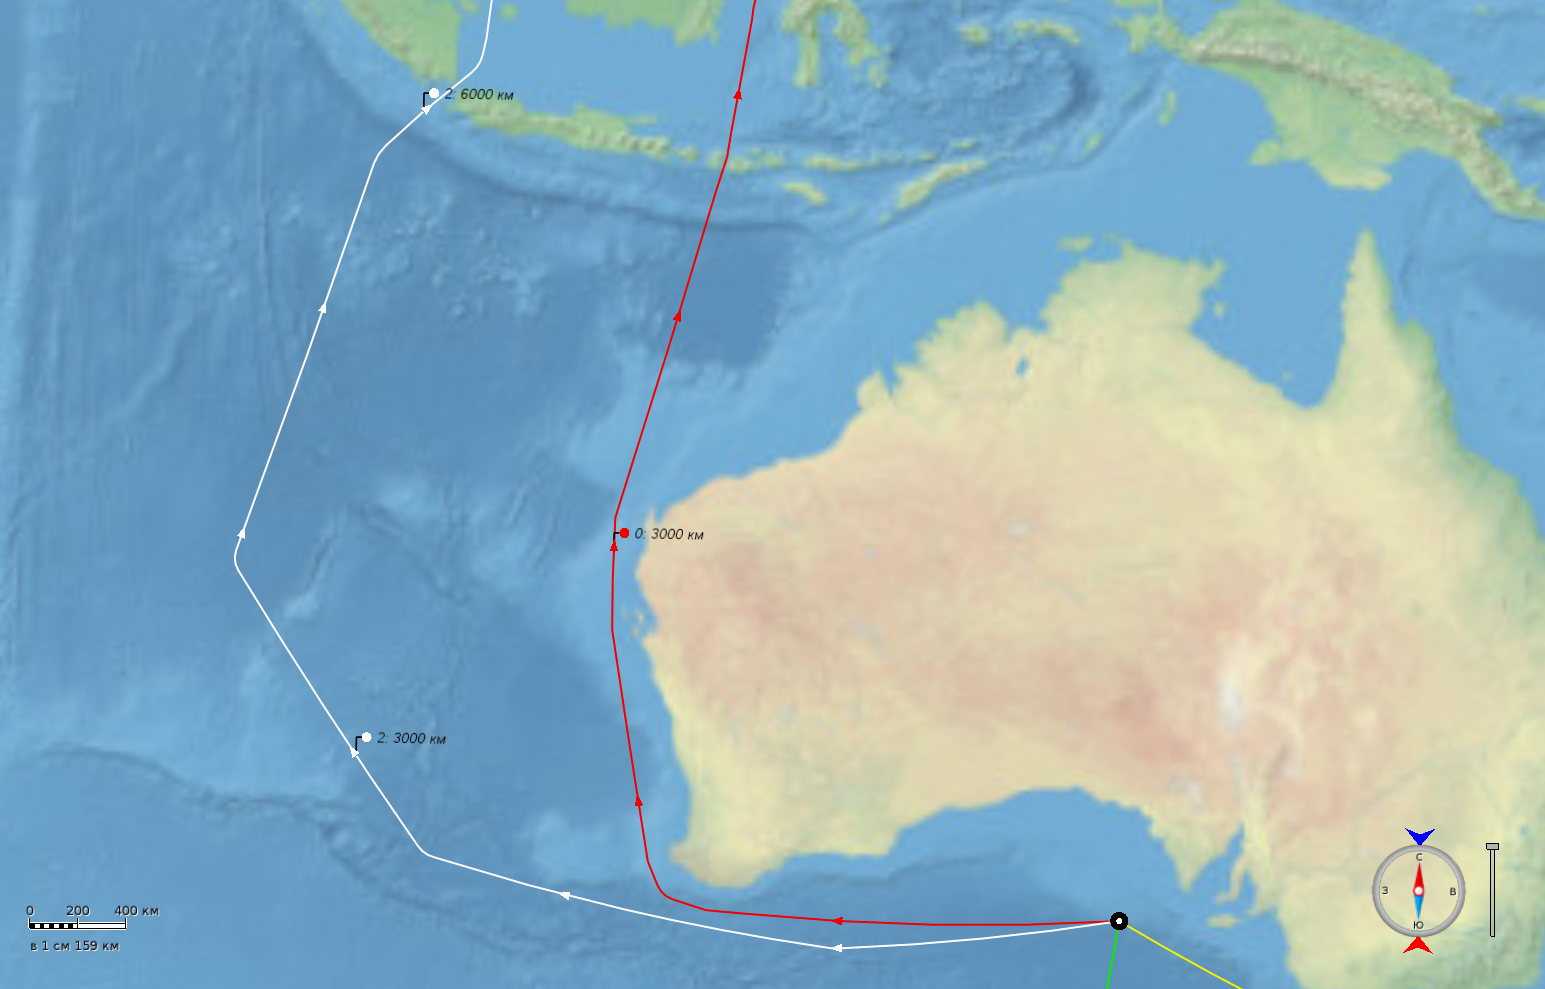
\includegraphics[width=\textwidth, clip=true, trim = 200 0 300
    0]{Solution/weights-on-path-bad}
    \caption{Маршруты несущественно разошлись}
    \label{fig:weights-on-path-bad}
\end{figure}

\begin{figure}
    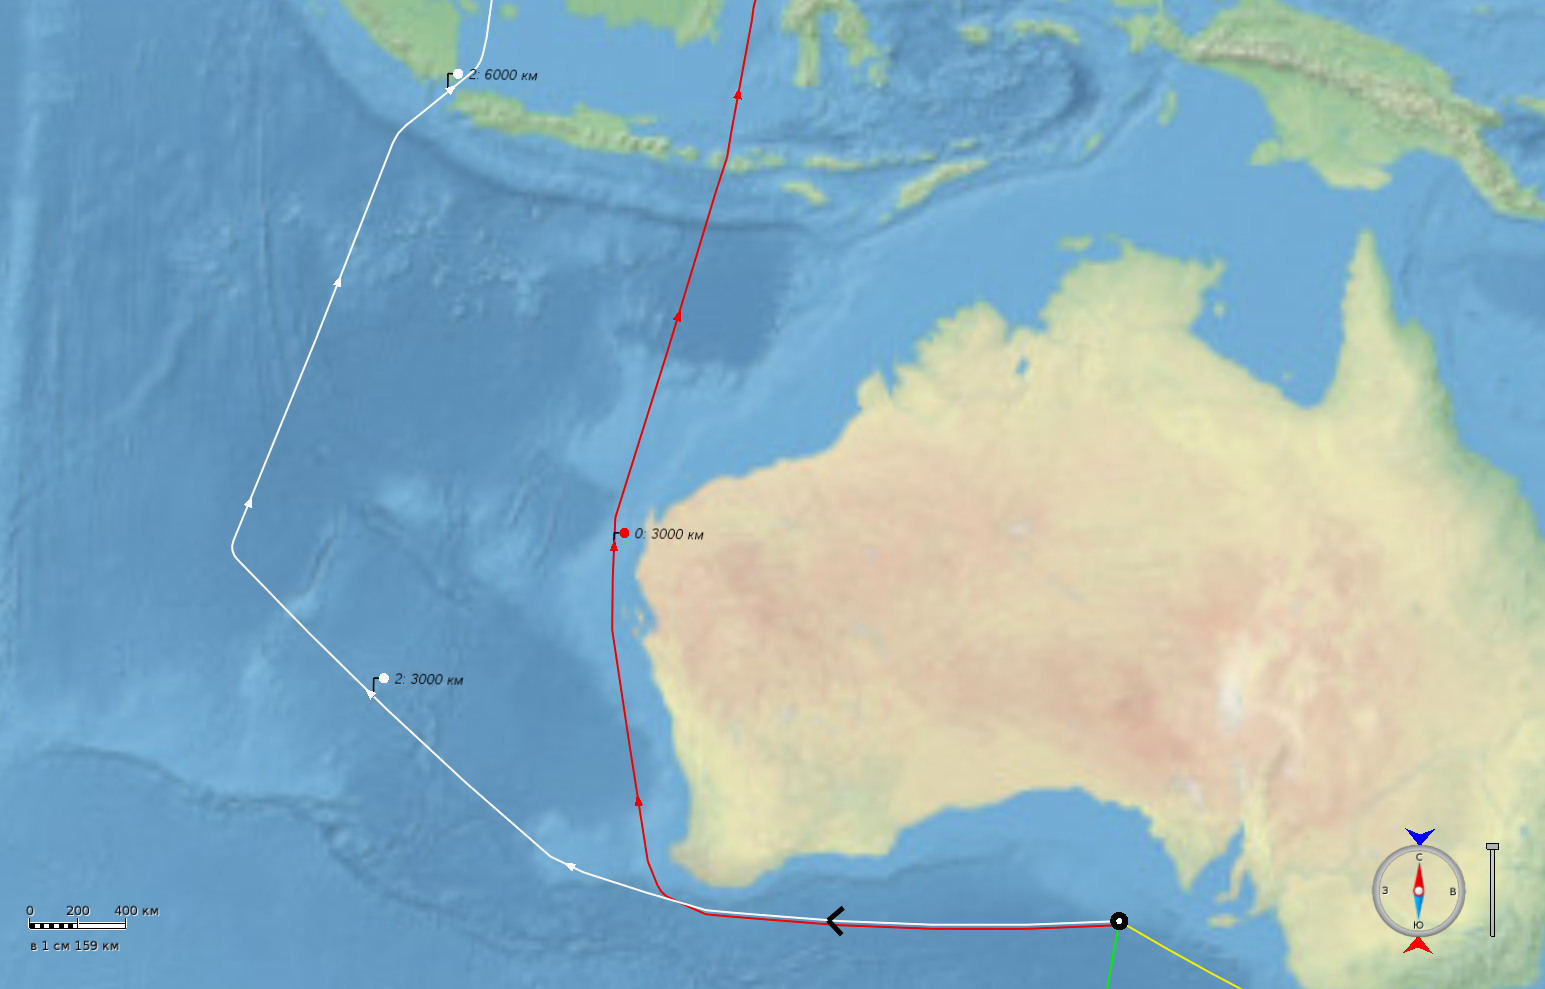
\includegraphics[width=\textwidth, clip=true, trim = 200 0 300
    0]{Solution/weights-on-path-good}
    \caption{Маршруты совпадают в начале}
    \label{fig:weights-on-path-good}
\end{figure}

Описанный выше способ обновления весов рёбер обладает недостатком,
проиллюстрированным на рисунке~\ref{fig:weights-on-path-bad}. Проблема
заключается в том, что для вершин найденного маршрута значение
потенциалов максимально (поскольку расстояние от фиктивной вершины
равно нулю). В связи с этим следующий найденный маршрут будет
проходить на небольшом расстоянии от предыдущего. При этом он станет
длиннее, но не станет непохожим в смысле сформулированного ранее
критерия. Разумеется, такое поведение является неестественным и не
удовлетворяет неформальной постановке задачи. Поэтому кратчайшие
расстояния от фиктивной вершины до вершин на маршруте принимаются
равными $\frac{limit}{M}$, где $M > 1$ --- параметр алгоритма. За счёт
этого южная часть белого маршрута совпала с той же частью красного,
проходящего по кратчайшему пути (рис.~\ref{fig:weights-on-path-good}).

\begin{figure}
    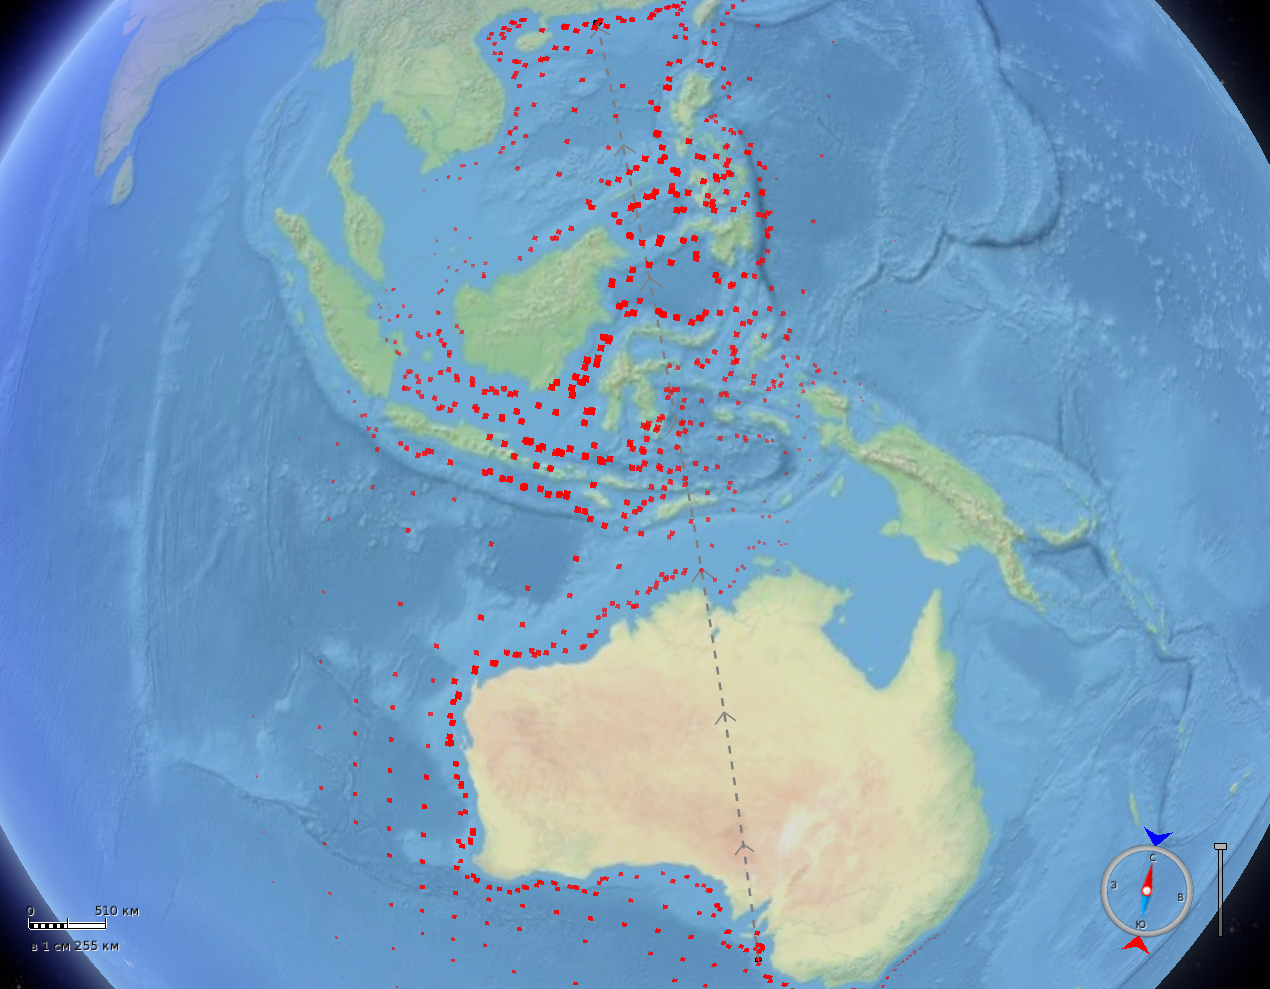
\includegraphics[width=\textwidth]{Solution/potentials-update/accum1}
    \caption{Обновление потенциалов: умножение (1)}
    \label{fig:update-accum1}
\end{figure}

\begin{figure}
    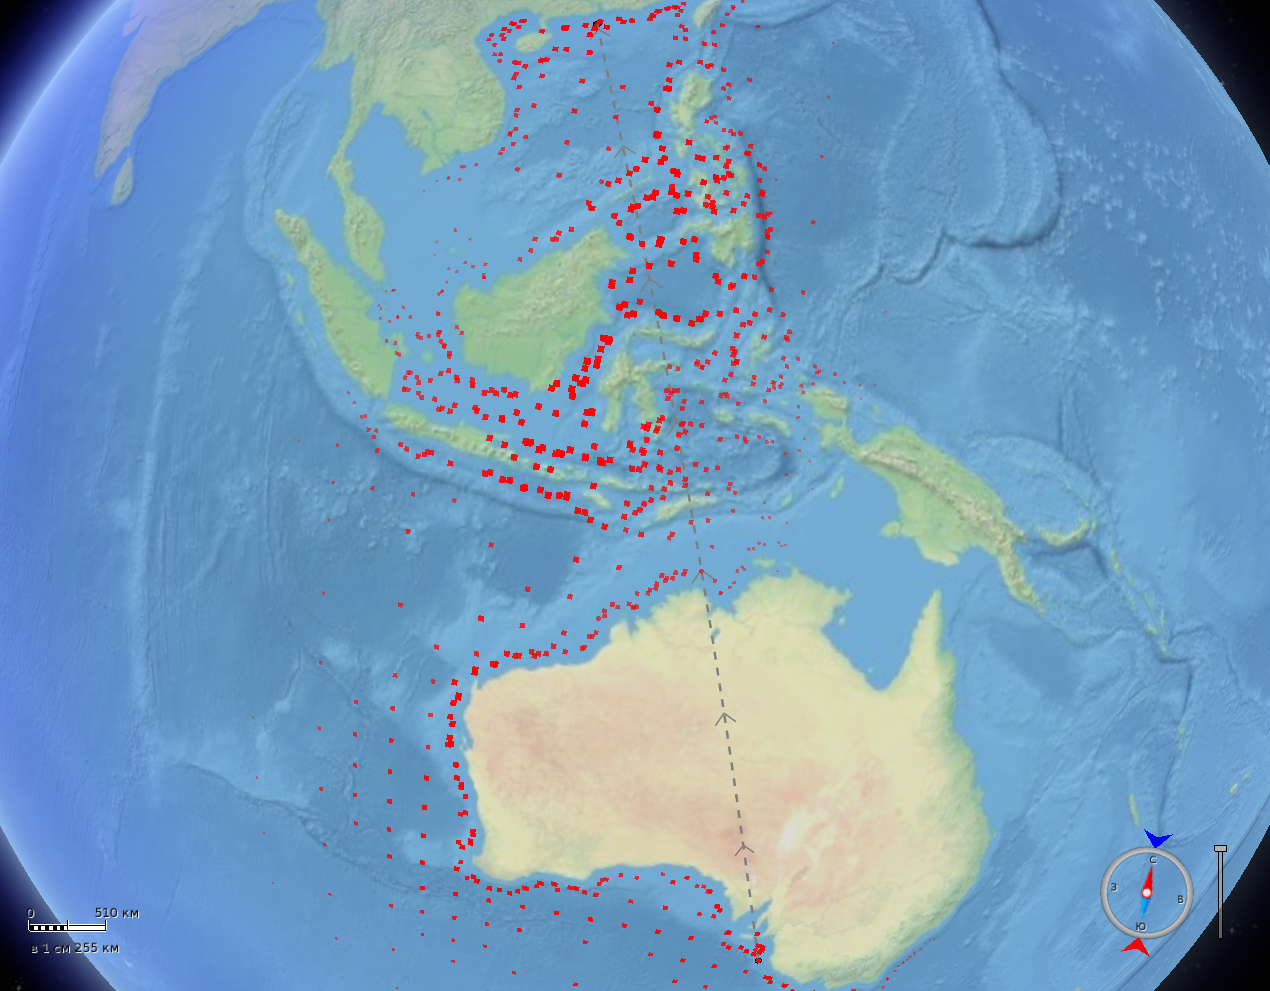
\includegraphics[width=\textwidth]{Solution/potentials-update/max1}
    \caption{Обновление потенциалов: максимум (1)}
    \label{fig:update-max1}
\end{figure}

\begin{figure}
    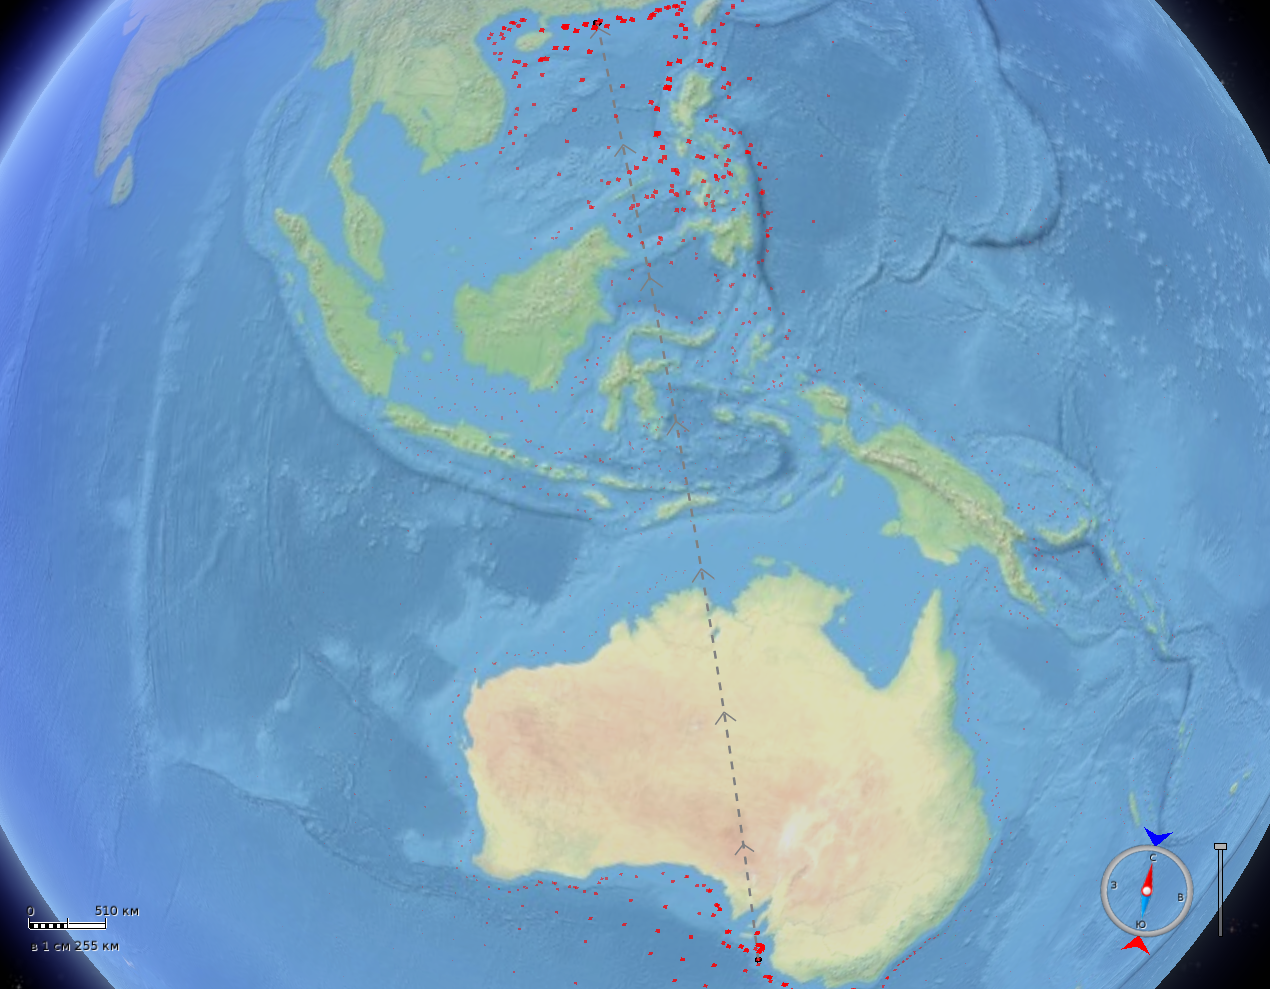
\includegraphics[width=\textwidth]{Solution/potentials-update/accum2}
    \caption{Обновление потенциалов: умножение (2)}
    \label{fig:update-accum2}
\end{figure}

\begin{figure}
    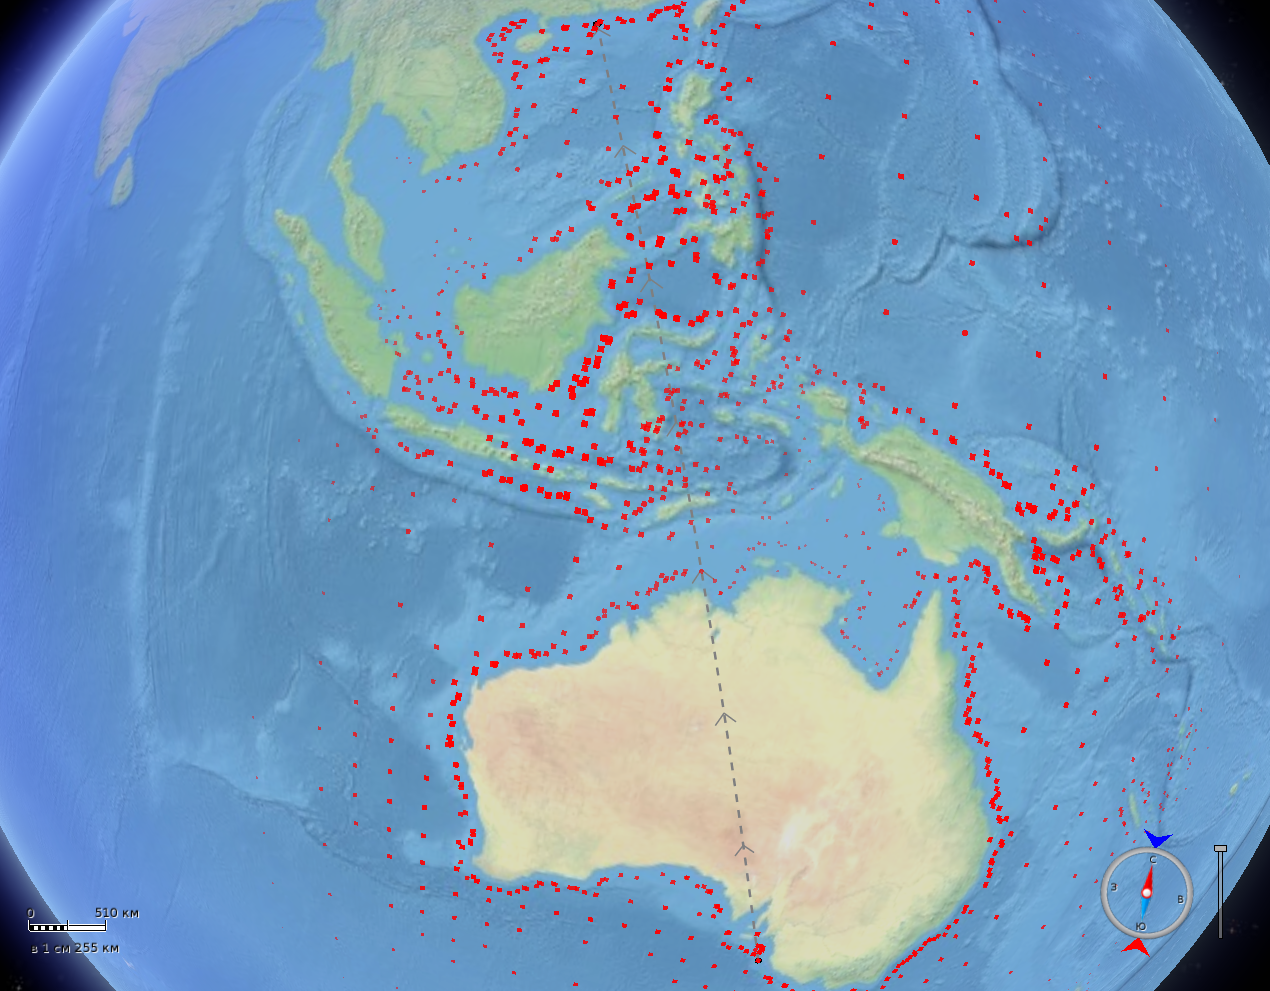
\includegraphics[width=\textwidth]{Solution/potentials-update/max2}
    \caption{Обновление потенциалов: максимум (2)}
    \label{fig:update-max2}
\end{figure}

\begin{figure}
    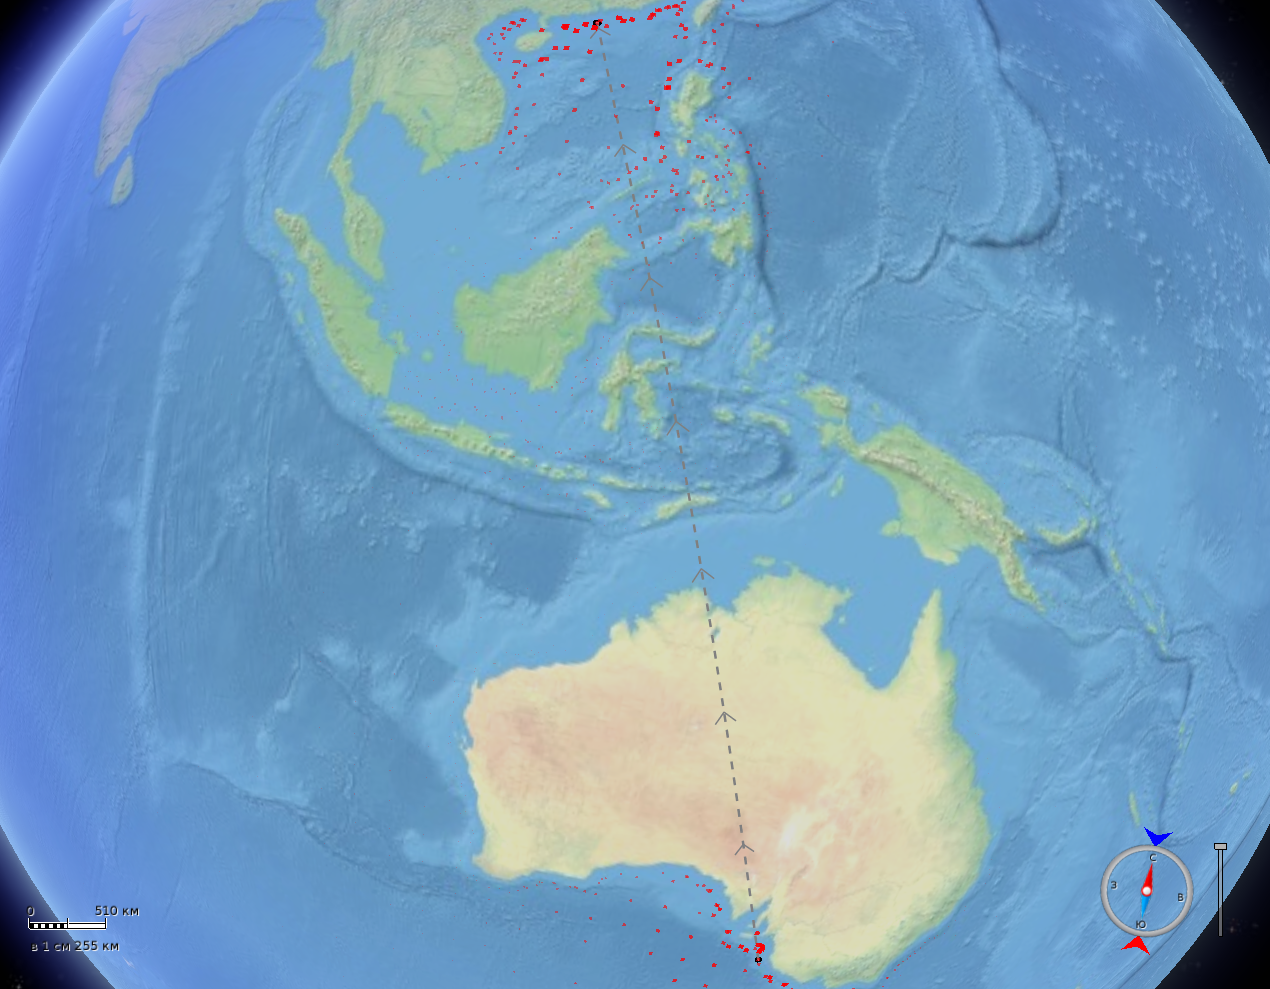
\includegraphics[width=\textwidth]{Solution/potentials-update/accum3}
    \caption{Обновление потенциалов: умножение (3)}
    \label{fig:update-accum3}
\end{figure}

\begin{figure}
    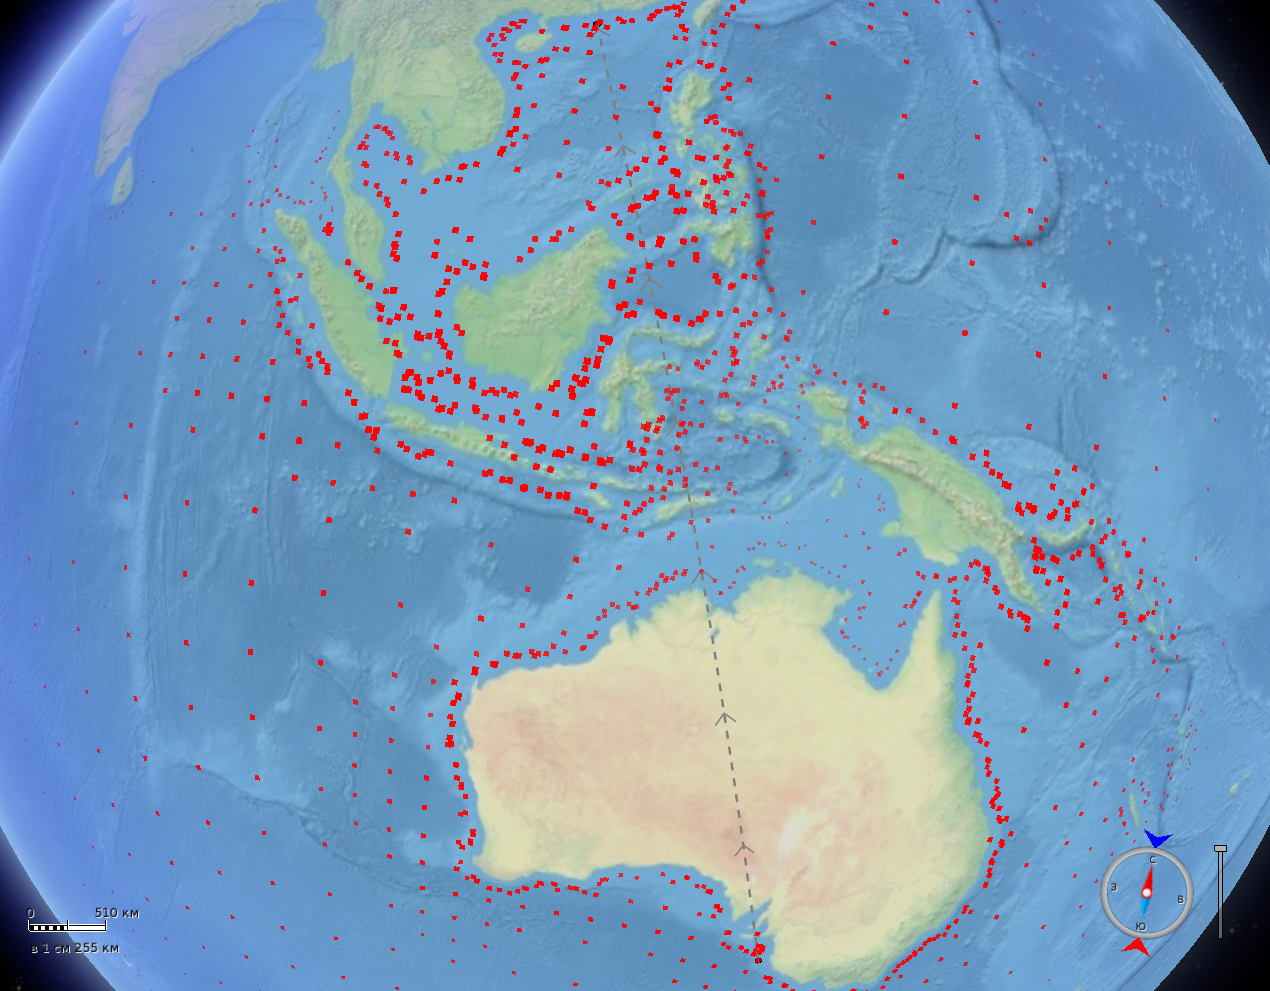
\includegraphics[width=\textwidth]{Solution/potentials-update/max3}
    \caption{Обновление потенциалов: максимум (3)}
    \label{fig:update-max3}
\end{figure}

\begin{figure}
    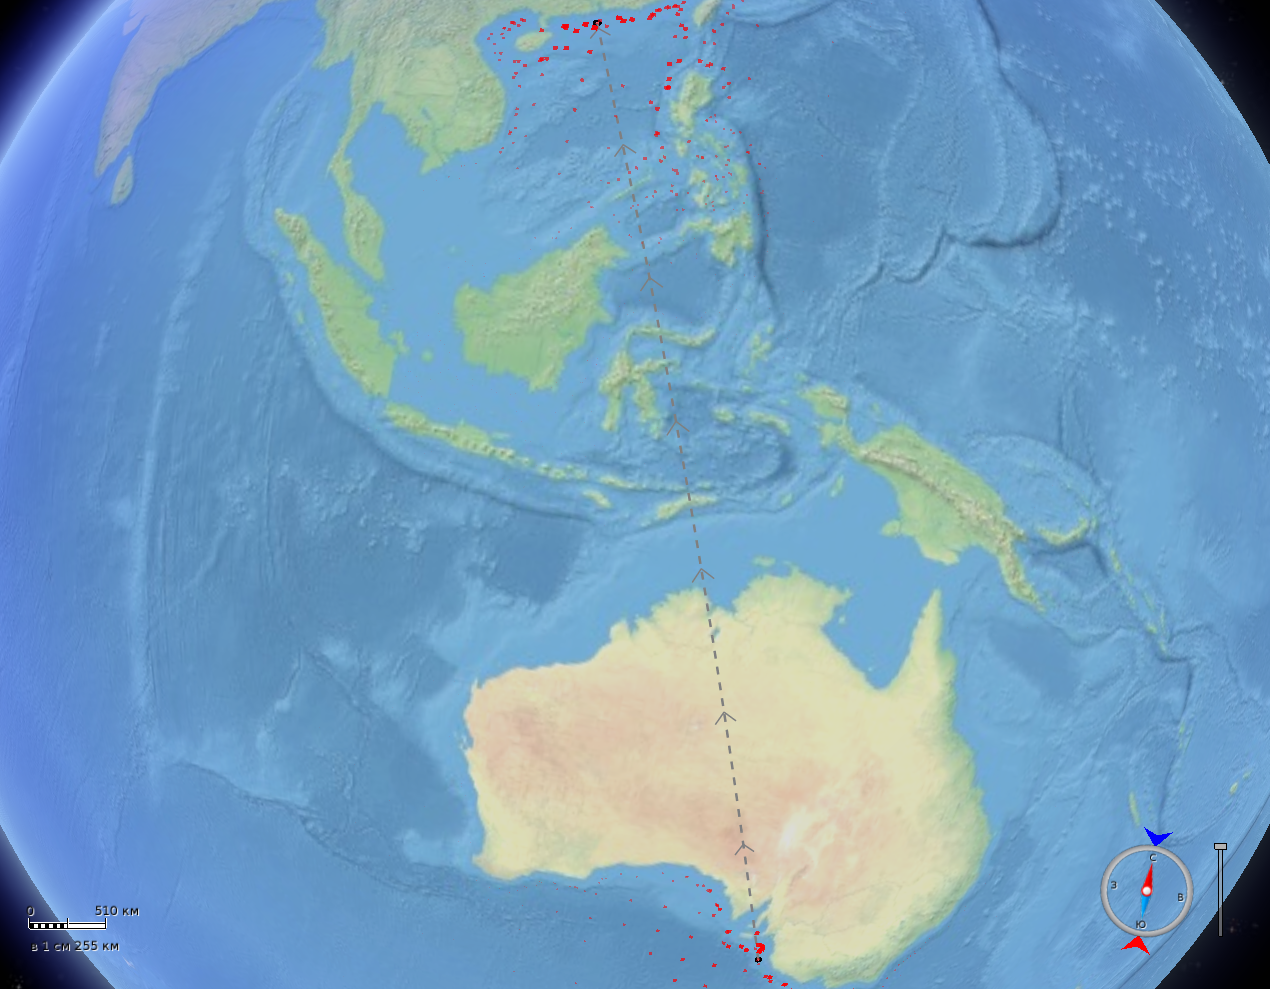
\includegraphics[width=\textwidth]{Solution/potentials-update/accum4}
    \caption{Обновление потенциалов: умножение (4)}
    \label{fig:update-accum4}
\end{figure}

\begin{figure}
    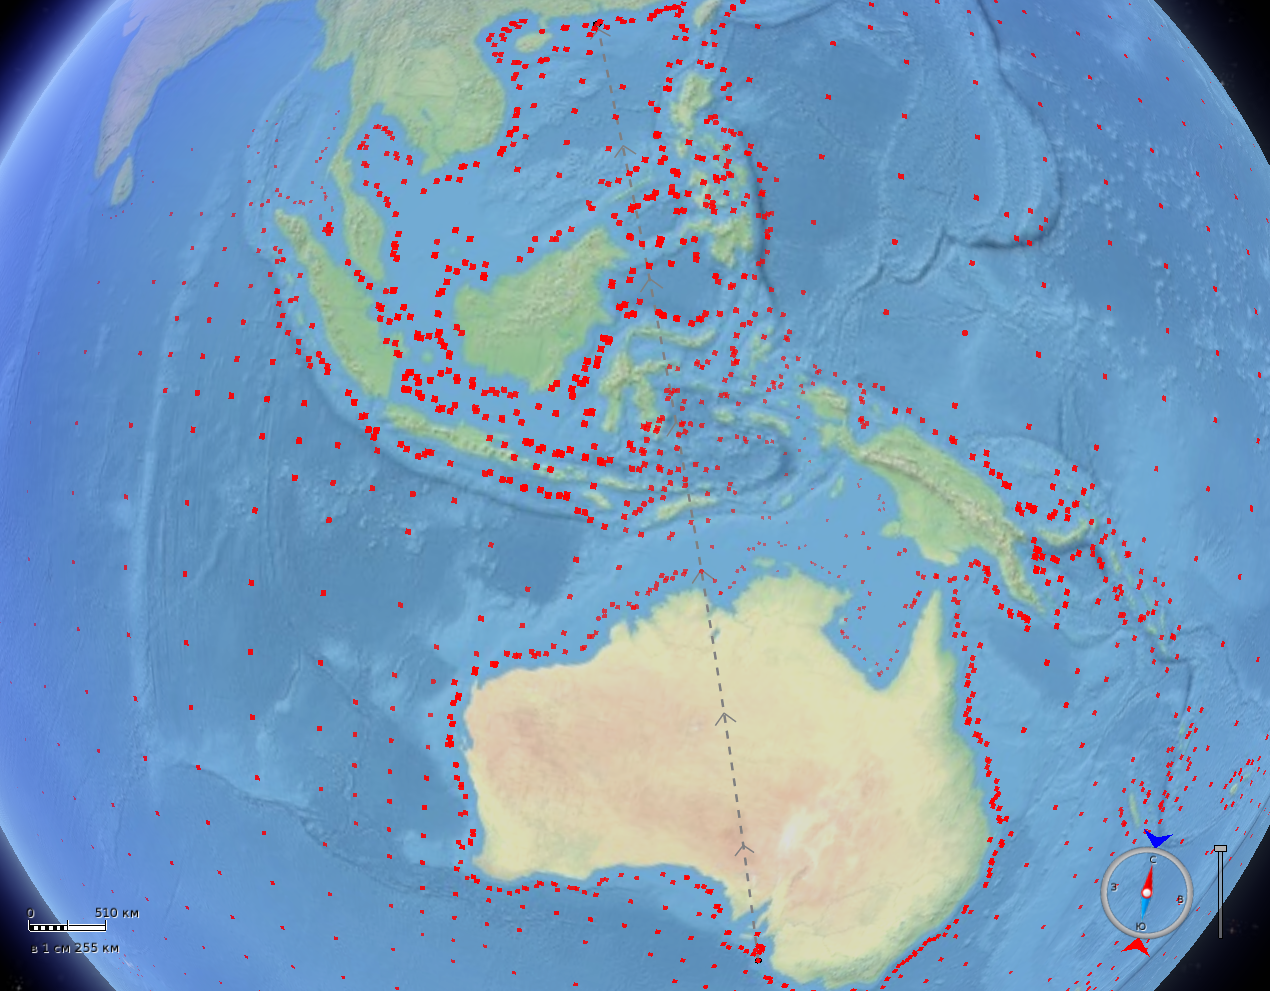
\includegraphics[width=\textwidth]{Solution/potentials-update/max4}
    \caption{Обновление потенциалов: максимум (4)}
    \label{fig:update-max4}
\end{figure}

\begin{figure}
    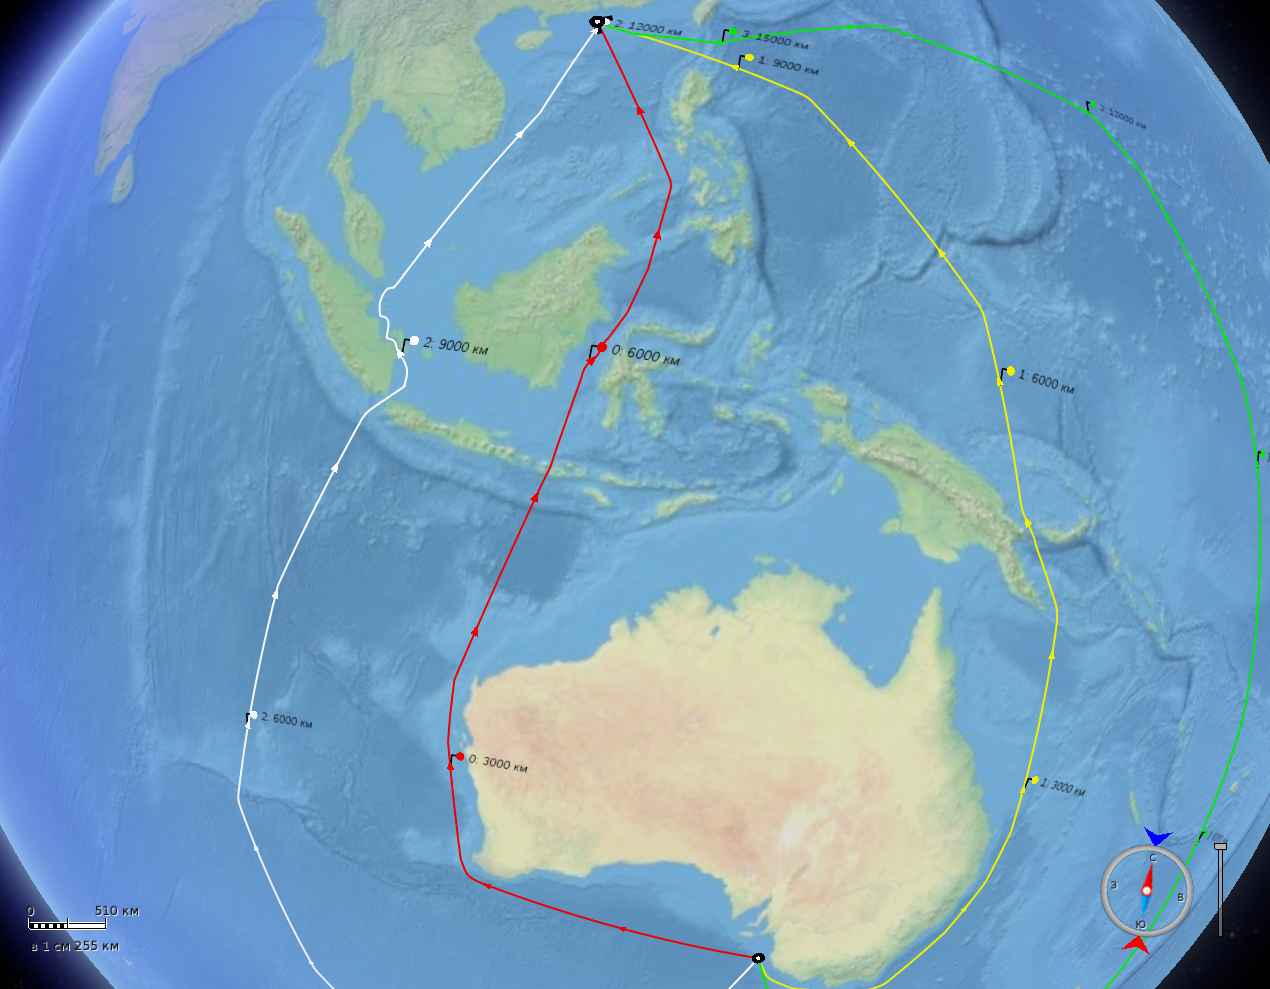
\includegraphics[width=\textwidth]{Solution/potentials-update/accum_result}
    \caption{Найденные маршруты при использовании умножения}
    \label{fig:update-accum-result}
\end{figure}

\begin{figure}
    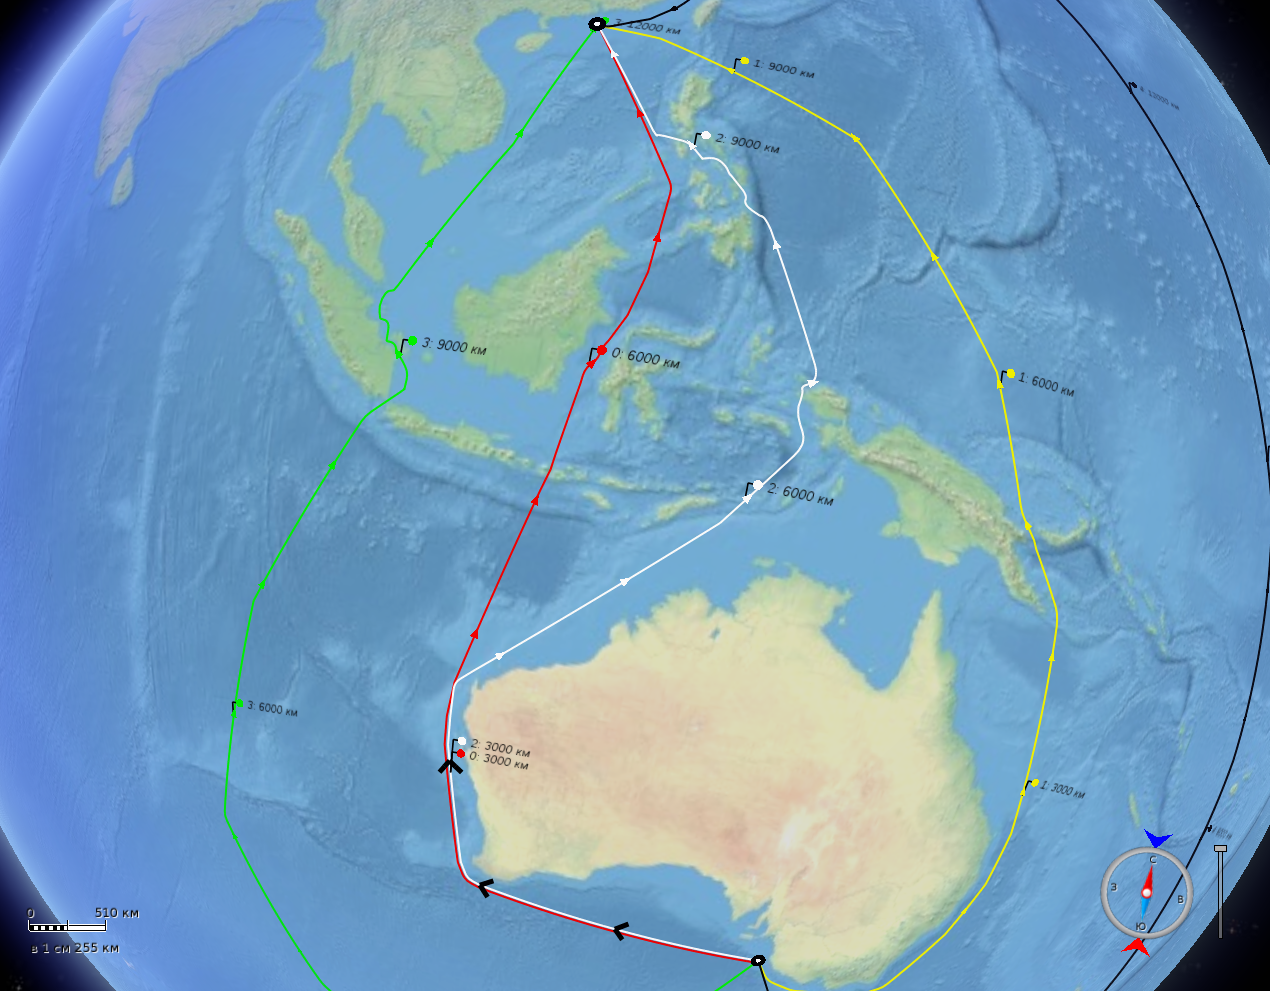
\includegraphics[width=\textwidth]{Solution/potentials-update/max_result}
    \caption{Найденные маршруты при использовании максимума}
    \label{fig:update-max-result}
\end{figure}

Наконец, последний вопрос состоит в обновлении потенциалов, после того
как найден очередной маршрут. Понятно, что потенциалы должны как-то
накапливаться, чтобы учитывать влияние всех предыдущих маршрутов и не
допускать прохождение нового маршрута вблизи старых. Например, можно
для каждой вершины в качестве нового потенциала брать сумму или
произведение имеющегося потенциала и вновь посчитанного. Также можно
брать максимум. На
рисунках~(\ref{fig:update-accum1}--\ref{fig:update-max4})
проиллюстрированы различия между двумя вариантами: перемножением и
максимумом. Красные квадраты визуализируют значения потенциалов: чем
больше и ярче квадрат, тем больше потенциал. После нахождения первого
маршрута потенциалы, очевидно, распределены одинаково
(рис.~\ref{fig:update-accum1} и \ref{fig:update-max1}). Затем, если
перемножать потенциалы, то для вершин в окрестностях начальной и
конечной точек они оказываются сильно больше, чем для остальных
вершин~(рис.~\ref{fig:update-accum2}). Если же брать максимум, то
распространение потенциалов происходит равномерно: во всех точках,
расположенных близко к какому-либо найденному маршруту, потенциал
оказывается большой~(\ref{fig:update-max2}).
Рисунки~(\ref{fig:update-accum3}--\ref{fig:update-max4})
демонстрируют, что в дальнейшим описанный эффект лишь усиливается. В
результате проведённого эксперимента при использовании максимума для
обновления потенциалов было найдено на один маршрут
больше~(рис.~\ref{fig:update-accum-res}--\ref{fig:update-max-res}).
Поэтому в предложенном алгоритме используется максимум для обновления
потенциалов.

\FloatBarrier

